% 2013 辽宁卷文科第 22 题：AB 为 ⊙O 直径，CD 切 ⊙O 于 E，AD⊥CD，BC⊥CD，EF⊥AB。
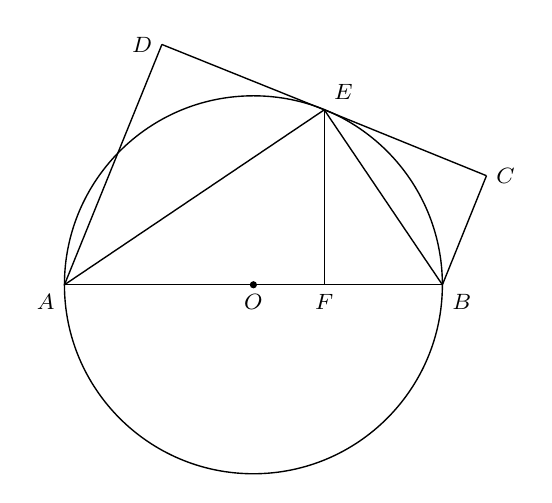
\begin{tikzpicture}[font=\footnotesize, line width=0.5pt, scale=1.0]
  \coordinate (O) at (0,0);
  \coordinate (A) at (-2.4,0);
  \coordinate (B) at (2.4,0);
  \coordinate (E) at (0.90,2.222);
  \coordinate (F) at (0.90,0);
  \coordinate (D) at (-1.162,3.052);
  \coordinate (C) at (2.960,1.385);
  % 圆
  \draw (O) circle (2.4);
  % 直径与切线
  \draw (A) -- (B);
  \draw (D) -- (E) -- (C);
  % 垂线
  \draw (A) -- (D);
  \draw (B) -- (C);
  \draw (E) -- (F);
  % 连接 AE、BE
  \draw (A) -- (E);
  \draw (B) -- (E);
  % 点与标签
  \fill (O) circle (1.3pt) node[below] {$O$};
  \node[below left] at (A) {$A$};
  \node[below right] at (B) {$B$};
  \node[above right] at (E) {$E$};
  \node[left] at (D) {$D$};
  \node[right] at (C) {$C$};
  \node[below] at (F) {$F$};
\end{tikzpicture}
